\providecommand\lcode{\begingroup \small\urlstyle{tt}\Url}
\providecommand\lident{\begingroup \small\urlstyle{tt}\Url}

\chapter{Propagating Information using SSA\Author{F. Brandner \andAuthor D. Novillo}}
\label{chapter:constant_propagation_is_easier}
\inputprogress
\newcommand{\obacht}[2]{\marginpar{\tiny\textbf{#1:} #2}}

\graphicspath{{img/}{constant_propagation_is_easier/img/}{part3/constant_propagation_is_easier/img/}}

\lstdefinelanguage{DNlisting}
{
  morekeywords={PHI,ASSERT_EXPR},
  morekeywords=[2]{struct,const,int,void,for,if,throw,call,return},
  sensitive=true,
%   morecomment=[s]{<!--}{-->},
%   morestring=[b]",
}

\lstset{
  mathescape=true,
  language=DNlisting,
  basicstyle=\small,
  keywordstyle=\ttfamily,
  keywordstyle=[2]\bfseries,
%   identifierstyle=,
%   stringstyle=\color{black}\ttfamily,
%   commentstyle=\it,
%   moredelim=[is][\color{MyDarkGreen}\ttfamily]{|}{|}
  numbers=left
}

\section{Overview}

A central task of compilers is to \emph{optimize} a given input program such
that the resulting code is more efficient in terms of execution time, code size,
or some other metric of interest. However, in order to perform these
optimizations, typically some form of \emph{program analysis} is
required to determine if a given program transformation is applicable, to
estimate its profitability, or to guarantee its correctness.

\emph{Data flow analysis}~\cite{novillo:bib:NNH99} is a simple, yet powerful,
approach to program analysis that is utilized by many compiler frameworks and
program analysis tools today. We will introduce the basic concepts of
traditional data flow analysis in this chapter and will show how the \emph{static
single assignment} form (SSA) facilitates the design and implementation of
equivalent analyses.
We will also show that how the SSA property allows us to reduce the compilation
time and memory consumption of the data flow analyses that this program
representation supports.

Traditionally, data flow analysis is performed on a \emph{control flow graph}
representation (CFG) of the input program. Nodes in the graph represent
operations and edges the potential flow of program execution.
Information on certain \emph{program properties} is propagated among
the nodes along the control flow edges until the computed information
stabilizes, i.e., no \emph{new} information can be inferred from the program.

The \emph{propagation engine} presented in the following sections is an
extension of the well known approach by Wegman and Zadeck for \emph{sparse
conditional constant propagation}~\cite{bib:wegman.ea-91} (also known as
SSA-CCP). Instead of using the CFG they represent the input program as an
\emph{SSA graph}~\cite{novillo:bib:cytron.ea-91}. Operations are again represented as
nodes in this graph, however, the edges represent \emph{data dependencies}
instead of control flow. This representation allows a selective propagation of
program properties among data dependent graph nodes only. As before, the
processing stops when the information associated with the graph nodes stabilizes.
The basic algorithm is not limited to constant propagation and can also be
applied to solve a large class of other data flow problems
efficiently~\cite{novillo:bib:N05}. However, not all data flow
analyses can be modeled. In this chapter we will also investigate the limitations
of the SSA-based approach.

The remainder of this chapter is organized as follows. First, the basic concepts
of (traditional) data flow analysis are presented in
Section~\ref{novillo:sec:preliminaries}. This will provide the theoretical
foundation and background for the discussion of the SSA-based propagation
engine in Section~\ref{novillo:sec:prop-engine}. We then provide an example of a
data flow analysis that can be performed efficiently by the aforementioned
engine, namely copy propagation in Section~\ref{novillo:sec:example}. We
conclude and provide links for further reading in
Section~\ref{novillo:sec:further_reading}.

%%%%%%%%%%%%%%%%%%%%%%%%%%%%%%%%%%%%%%%%%%%%%%%%%%%%%%%%%%%%%%%%%%%%%%%%%%%%%%%%
\section{Preliminaries}
\label{novillo:sec:preliminaries}

Data flow analysis is at the heart of many compiler transformations and
optimizations, but also finds application in a broad spectrum of analysis and
verification tasks in program analysis tools such as program checkers, profiling
tools, and timing analysis tools. This section gives a brief introduction to the
basics of data flow analysis. Due to space considerations, we cannot cover this
topic in full depth.

As noted before, data flow analysis derives information from certain
interesting program properties that may help to optimize the program. Typical
examples of interesting properties are: the set of \emph{live} variables at a
given program point, the particular constant value a variable may take, or the
set of program points that are reachable at run-time. Liveness information, for
example, is critical during register allocation, while the two latter properties
help to simplify computations and to identify dead code.

The analysis results are gathered from the input program by propagating
information among its operations considering all potential execution paths. The
propagation is typically performed iteratively until the computed results
stabilize. Formally, a data flow problem can be specified using a \emph{monotone
framework} that consists of:
\begin{itemize}
  \item a \emph{complete lattice} representing the property space,
  \item a \emph{flow graph} resembling the control flow of the input program, 
        and
  \item a set of \emph{transfer functions} modeling the effect of individual
        operations \\ on the property space.
\end{itemize}

%///////////////////////////////////////////////////////////////////////////////
\textbf{Property Space:}
A key concept for data flow analysis is the representation of the property space
via \emph{partially ordered sets} $(L, \sqsubseteq)$, where $L$ represents some
interesting program property and $\sqsubseteq$ represents a reflexive, transitive, and
anti-symmetric relation. Using the $\sqsubseteq$ relation, \emph{upper} or
\emph{lower bounds}, as well as \emph{least upper} and \emph{greatest lower
bounds}, can be defined for subsets of $L$.

A particularly interesting class of partially ordered sets are \emph{complete
lattices}, where all subsets have a least upper bound as well as a greatest
lower bound. These bounds are unique and are denoted by $\bigsqcup$ and
$\bigsqcap$ respectively. In the context of program analysis the former is often
referred to as the \emph{join operator}, while the latter is termed the
\emph{meet operator}. Complete lattices have two distinguished elements, the
\emph{least element} and the \emph{greatest element}, often denoted by $\bot$
and $\top$ respectively.

An \emph{ascending chain} is a totally ordered subset $\{l_1, \ldots, l_n \}$ of
a complete lattice. A chain is said to \emph{stabilize} if there exists an index
$m$, where $\forall i > m \colon l_i = l_m$. An analogous definition can be
given for \emph{descending chains}.

%///////////////////////////////////////////////////////////////////////////////
\textbf{Program Representation:}
The functions of the input program are represented as control flow graphs, where
the nodes represent operations, or instructions, and edges denote the potential
flow of execution at run-time.
Data flow information is then propagated from one node to
another adjacent node along the respective graph edge using \emph{in} and
\emph{out} sets associated with every node. If there exists only one edge
connecting two nodes, data can be simply copied from one set to the other.
However, if a node has multiple incoming edges, the information from
those edges has to be combined using the meet or join operator.

Sometimes, it is helpful to reverse the flow graph to propagate information,
i.e., reverse the direction of the edges in the control flow graph. Such
analyses are termed \emph{backward analyses}, while those using the
regular flow graph are \emph{forward analyses}.

%///////////////////////////////////////////////////////////////////////////////
\textbf{Transfer Functions:}
Aside from the control flow, the operations of the program
need to be accounted for during analysis.
Usually these operations change the way data is propagated from one control
flow node to the other. Every operation is thus mapped
to a \emph{transfer function}, which transforms the information available from
the \emph{in} set of the operation's flow graph node and stores the result in
the corresponding \emph{out} set.

%///////////////////////////////////////////////////////////////////////////////
\subsection{Solving Data Flow Problems}

Putting all those elements together, i.e., a complete lattice, a flow graph, and
a set of transfer functions, yields an instance of a monotone framework.
This framework describes a set of \emph{data flow equations} whose solution will
ultimately converge to the solution of the data flow analysis. A very popular and
intuitive way to solve these equations is to compute the \emph{maximal (minimal) fixed point}
(MFP) using
an iterative work list algorithm. The work list contains edges of the flow graph
that have to be revisited by first combining the information from the \emph{out}
set of the edge's source node with the \emph{in} set of the edge's target node
using the meet or join operator, then applying the transfer function of the
target node, and finally propagating the obtained information to all successors
of the target node by appending them to the work list. The algorithm terminates
when the data flow information stabilizes and the work list becomes empty.

It is obvious that a single flow edge can be appended several times to the
work list in the course of the analysis. It may even happen that an infinite
feedback loop prevents the algorithm from terminating. We are thus interested in
bounding the number of times a flow edge is processed. Recalling the definition
of chains from before, % FERNANDO: could you cite the chapter?
 the \emph{height} of a
lattice is defined by the length of its longest chain. We can ensure termination
for lattices fulfilling the \emph{ascending chain condition}, which ensures that
the lattice has finite height. Given a lattice with finite height $h$ and a flow
graph $G~=~(V,~E)$ it is easy to see that the MFP solution can be computed in
$O(|E| \cdot h)$ time, where $|E|$ represents the number of edges. Since the
number of edges is bounded by the number of graph nodes $|V|$,
i.e., $|E| \leq |V|^2$, this gives an $O(|V|^2 \cdot h)$ general algorithm to
solve data flow analyses. Note that the height of
the lattice often depends on properties of the input program, which might
ultimately yield bounds worse than cubic in the number of graph nodes. For
instance, for copy propagation the lattice consists of the cross product of many
smaller lattices, each representing the potential values of a variable occurring
in the program. The total height of the lattice thus directly depends on the
number of variables in the program.

% FERNANDO: this paragraph is a bit out of place here. If the reader stumbles
% on it for the first time, it will not be able to understand why these sets
% must be complete (and I think this is not a requirement, even in dense
% analysis) even if unrelated to the node where they are stored.
In terms of memory consumption, every node of the flow graph is associated with
complete \emph{in} and \emph{out} sets, where the stored information is
often unrelated to the particular graph node and only needed to propagate the
data flow information to all relevant program points.

%%%%%%%%%%%%%%%%%%%%%%%%%%%%%%%%%%%%%%%%%%%%%%%%%%%%%%%%%%%%%%%%%%%%%%%%%%%%%%%%
\section{Data Flow Propagation under SSA Form}
\label{chapter:constant_propagation_is_easier:sec:prop-engine}
\label{sec:prop-engine}

SSA form allows to solve a large class of data flow problems more efficiently
than the standard fixed point solution presented previously.
% FERNANDO: SSA-based algorithms also rely on the fix-point theory. I guess
% what you guys want to say is: "than the previous approach to data flow
% analyses."
The basic idea is to directly propagate information computed at the unique
definition of a variable to all its uses. In this way, intermediate program
points that neither define nor use the variable of interest do not have to
be taken into consideration; thus, reducing memory consumption
and compilation time.

%///////////////////////////////////////////////////////////////////////////////
\subsection{Program Representation}

% FENRANDO: This paragraph is unnecessary, and actually repetitive:
% phi-functions have already been defined, and are discussed all over the book.
Programs in SSA form exhibit, aside from the regular operations of the original
program, special operations called $\phi$-operations, which are placed at join
points of the original CFG. In the following, we assume that possibly many
$\phi$-operations are associated with the corresponding CFG nodes at those
join points.

Data flow analyses under SSA form rely on a specialized program representation
based on \emph{SSA graphs}, which resemble traditional \emph{def-use chains} and
simplify the propagation of data flow information. The nodes of an SSA graph
correspond to the operations of the program, including the program's
$\phi$-operations that are represented by dedicated nodes in the graph. The
edges of the graph connect the unique definition of a variable with all its
uses, i.e., edges represent true dependencies.

The SSA graph captures, besides the data
dependencies, the \emph{relevant} join points of the program's CFG. A join point
is relevant for the analysis, whenever the value of two or more definitions may
reach a use by passing through that join. The SSA form properties ensure that
a $\phi$-operation is placed at the join point and that any use of the variable
that the $\phi$-function defines has been properly updated to refer to the
correct name.

\begin{figure}[t]
  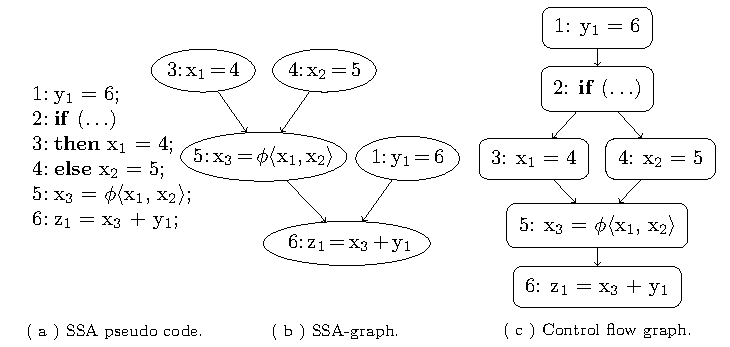
\includegraphics[trim=4.3mm 0 0 0]{ssa_graph}
  \caption{Example program and its SSA graph.}
  \label{novillo:fig:ssa_graph}
\end{figure}

% FERNANDO: I am not sure, but I think 'allow' with the meaning of permit, is
% normally transitive, with two objects, e.g., the graph allows <the analysis>
% <to do something>.
Consider for example, the code excerpt shown in
Figure~\ref{novillo:fig:ssa_graph}, along with the corresponding SSA graph and
CFG. Assume we are interested in propagating information from the assignment of
variable y$_1$, at the beginning of the code, down to its unique use at
the end. The traditional CFG representation causes the propagation
to pass through several intermediate program points. These program points are
concerned with computations of the variables x$_1$, x$_2$, and x$_3$ only and
are thus irrelevant for the computation. The SSA graph representation, on
the other hand, propagates the desired information directly from definition to
use sites, without
any intermediate steps. At the same time, we also find that the control flow
join, following the \textbf{if}, is properly represented by the $\phi$-operation
defining the variable x$_3$ in the SSA graph.

Even though the SSA graph captures data dependencies and the relevant join
points in the CFG, it lacks information on other
\emph{control dependencies}. However, analysis results can often be improved
significantly by considering the additional information that is available from
the control dependencies in the program's CFG. As an example consider, once more,
the code excerpt shown in Figure~\ref{novillo:fig:ssa_graph}. Assume that the
condition associated with the \textbf{if} operation is known to be false for all
possible program executions. Consequently, the $\phi$-operation will select the
value of x$_2$ in all cases, which is known to be of constant value $5$.
However, due to the shortcomings of the SSA graph this information cannot be
derived. It is thus important to use both, the control flow graph and the SSA
graph, during data flow analysis in order to obtain the best possible results.

%///////////////////////////////////////////////////////////////////////////////
\subsection{Sparse Data Flow Propagation}

\begin{algorithm}[t!]
  \begin{enumerate}
    \item Initially, every edge in the CFG is marked not executable and the
          \emph{CFGWorkList} is seeded with the outgoing edges of the control
          flow graph's \emph{start} node.  The \emph{SSAWorkList} is empty.
    \item \label{novillo:alg:propagation:loop} Remove the top element of either
          of the two work lists.
    \item \label{novillo:alg:propagation:flowedge} If the element is a control
          flow edge that is marked to be executable, do nothing, \\
          otherwise proceed as follows:
          \begin{itemize}
            \vspace{-1.2ex}
            \item Mark the edge as executable.
            \item Visit every $\phi$-operation associated with the edge's target
                  node.
            \item When the target node was reached the first time via the
                  \emph{CFGWorkList} visit its operation.
            \item When the target node has a single outgoing non-executable edge
                  append that edge to the \emph{CFGWorkList}.
          \end{itemize}
          \vspace{-1ex}
    \item \label{novillo:alg:propagation:ssaedge} If the element is an edge from
          the SSA graph, process the target operation as follows:
          \begin{enumerate}
            \vspace{-1.2ex}
            \item[a.] When the target operation is a $\phi$-operation visit that
                      $\phi$-operation.
            \item[b.] \label{novillo:alg:propagation:ssaedge:regular} For
                      regular target operations, examine the corresponding
                      executable flag of the incoming edges of its corresponding
                      control flow graph node. If any of those edges is marked
                      executable visit the operation, otherwise do nothing.
          \end{enumerate}
          \vspace{-1ex}
    \item Continue with step \ref{novillo:alg:propagation:loop} until both work
          lists become empty.
  \end{enumerate}

  \caption{Sparse Data Flow Propagation}
  \label{alg:constant_propagation_is_easier:propagation}
\end{algorithm}

Similar to monotone frameworks for traditional data flow analysis, frameworks
for \emph{sparse data flow propagation} under SSA form can be defined using:
\begin{itemize}
  \item a \emph{complete lattice} representing the property space,
  \item a set of \emph{transfer functions} for the operations of the program,
  \item a \emph{control flow graph} capturing the program's execution flow, and
  \item an \emph{SSA graph} representing data dependencies.
\end{itemize}
We again seek a maximal (minimal) fixed point solution (MFP) using an iterative
work list
algorithm. However, in contrast to the algorithm described before, data flow
information is not propagated along the edges of the control flow graph but
along the edges of the SSA graph. For regular uses the propagation is then
straightforward due
to the fact that every use receives its value from a unique definition. Special
care has to be taken only for $\phi$-operations, which select a value among
their operands depending on the incoming control flow edges. The data flow
information of the
incoming operands has to be combined using the meet or join operator of the
lattice. As data flow information is propagated along SSA edges that have a
single source, it is sufficient to store the data flow information with the SSA
graph
node. The \emph{in} and \emph{out} sets used by the traditional approach -- see
Section~\ref{novillo:sec:preliminaries} -- are obsolete, since
$\phi$-operations already provide the required buffering.
% FERNANDO: this is not clear to me: I think these sets are no longer necessary
% because you can bind their info directly to the variables that they represent. % They would not be necessary even in a straight line program without phis.
In addition, the
control flow graph is used to track which operations are not reachable under any
program execution and thus can be ignored safely during the computation of the
fixed point solution.

The algorithm processes two work lists, the \emph{CFGWorkList}, containing edges
of the control flow graph, and the \emph{SSAWorkList}, which consists of edges
from the
SSA graph. It proceeds by removing the top element of either of those lists and
processing the respective edge as indicated by
Algorithm~\ref{alg:constant_propagation_is_easier:propagation}. Throughout the algorithm, operations of
the program are visited to update the work lists and propagate
information as shown in Algorithm~\ref{novillo:alg:visit}. We will highlight
the most relevant steps of the algorithms in more detail in the following
paragraphs.

\begin{algorithm}[t!]
  \begin{enumerate}
    \item Compute the operation's data flow information:
    \begin{enumerate}
      \vspace{-1.2ex}
      \item[a.] \label{novillo:alg:visit:phi} If the operation is a
                $\phi$-operation, combine the data flow information from all its
                operands where the corresponding control flow edge is marked 
                executable.
      \item[b.] \label{novillo:alg:visit:branch} In the case of conditional
                branches, update the operation's data flow information. Determine
                which of the outgoing control flow edges are reachable from the
                corresponding control flow graph node by examining the branch's
                condition(s) and append the respective non-executable edges to
                the \emph{CFGWorkList}.
      \item[c.] \label{novillo:alg:visit:regular} For regular operations, update
                the corresponding data flow information by applying its transfer
                function.
    \end{enumerate}
    \vspace{-1ex}
    \item Whenever the data flow information changes, append all outgoing edges
          of the corresponding SSA graph node to the \emph{SSAWorkList}.
  \end{enumerate}
  \caption{Visiting an Operation}
  \label{novillo:alg:visit}
\end{algorithm}

% FERNANDO: in my opinion the description of the algorithm is hard to follow.
% I think the main difficulty steams from the size of the sentences. They are
% very long, with many clauses on the same sentence.
In step~\ref{novillo:alg:propagation:flowedge} of the main algorithm, control
flow edges set as executable for the first time are processed.
Whenever such a control flow edge is processed, all
$\phi$-operations of its target node need to be reevaluated due to the fact that
Algorithm~\ref{novillo:alg:visit}a discarded the respective operands of the
$\phi$-operations so far -- because the control flow edge was not yet marked
executable.
Similarly, the operation of the target node has to be evaluated when the target
node is encountered to be executable for the first time, i.e., the currently
processed control flow edge is the first of its incoming edges that is marked
executable. Note that this is only required the \emph{first} time the node is
encountered to be executable, due to the processing of operations in
Step~\ref{novillo:alg:propagation:ssaedge}b, which thereafter triggers the
reevaluation automatically when necessary through the SSA graph.

Regular operations as well as $\phi$-operations are visited by
Algorithm~\ref{novillo:alg:visit} when the corresponding control flow graph node
has become executable or whenever the data flow information of one of their
predecessors in the SSA graph changed. At \linebreak $\phi$-operations the
information
from multiple control flow paths is combined using the usual meet or join
operator. However, only those operands where the associated control flow edge is
marked executable are considered. Conditional
branches are handled by examining its conditions based on the data flow
information computed so far. Depending on whether those conditions are
satisfiable or not, control flow edges are appended to the \emph{CFGWorkList} 
to ensure that all reachable operations are considered during the analysis.
Finally, all regular operations are processed by applying the relevant transfer
function and possibly propagating the updated information to all uses by
appending the respective SSA graph edges to the \emph{SSAWorkList}.

\begin{figure}[t]
  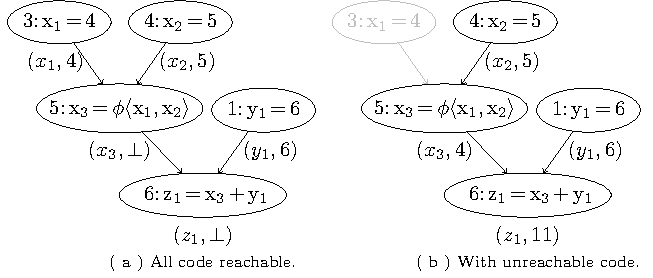
\includegraphics{ssa_propagation}
  \subfloat{\label{fig:constant_propagation_is_easier:ssa_propagation:a}}
  \subfloat{\label{fig:constant_propagation_is_easier:ssa_propagation:b}}
  \caption{Sparse conditional data flow propagation using SSA graphs.}
  \label{fig:constant_propagation_is_easier:ssa_propagation}
\end{figure}

As an example, consider the program shown in Figure~\ref{novillo:fig:ssa_graph}
and the constant propagation problem. First,
assume that the condition of the \textbf{if} cannot be statically evaluated, we
thus have to assume that all its successors in the CFG are reachable.
Consequently, all control flow edges in the program will eventually be marked
executable. This will trigger the evaluation of the constant assignments to
the variables x$_1$,  x$_2$, and y$_1$. The transfer functions immediately yield
that the variables are all constant, holding the values $4$, $5$, and $6$
respectively. This new information will trigger the reevaluation of the
$\phi$-operation of variable x$_3$. As both of its incoming control flow edges
are marked executable, the combined information yields $4 \bigsqcap 5 = \bot$,
i.e., the value is known not to be a particular constant value. Finally, also
the assignment
to variable z$_1$ is reevaluated, but the analysis shows that its value is not a
constant as depicted by Figure~\ref{fig:constant_propagation_is_easier:ssa_propagation:a}. If, however,
the condition of the \textbf{if} is known to be false for all possible program
executions a more precise result can be computed, as shown in
Figure~\ref{fig:constant_propagation_is_easier:ssa_propagation:b}. Neither the control flow edge
leading to the
assignment of variable~x$_1$ is marked executable nor its outgoing edge leading
to the $\phi$-operation of variable~x$_3$. Consequently, the reevaluation of
the $\phi$-operation considers the data flow information of its second operand
x$_2$ only, which is known to be constant. This enables the analysis
to show that the assignment to variable~z$_1$ is, in fact, constant as well.

%///////////////////////////////////////////////////////////////////////////////
\subsection{Discussion}

During the course of the propagation algorithm, every edge of the SSA graph is
processed at least once, whenever the operation corresponding to its definition
is found to be executable. Afterward, an edge can be revisited several times
depending on the height $h$ of the lattice representing the analysis' property
space. Edges of the control flow graph, on the other hand, are processed at most
once. This leads to an upper bound in execution time of $O(|E_{SSA}| \cdot h +
|E_{CFG}|)$, where $E_{SSA}$ and $E_{CFG}$ represent the edges of the SSA graph
and the control flow graph respectively. The size of the
SSA graph increases with respect to the original non-SSA program. Measurements
indicate that this growth is linear, yielding a
bound that is comparable to the bound of traditional data flow analysis.
However, in practice the SSA-based propagation engine outperforms the
traditional approach. This is  due to the direct propagation from the definition
of a variable to its uses, without the costly intermediate steps that have to be
performed on the CFG. The overhead is also reduced in terms of memory
consumption. Instead of storing the \emph{in} and \emph{out} sets capturing the
complete property space on every program point, it is sufficient to
associate every node in the SSA graph with the data flow information of the
corresponding variable only. This leads to considerable savings in practice.

%///////////////////////////////////////////////////////////////////////////////
\subsection{Limitations}

Unfortunately, the presented approach also has its limitations, which arise from
two sources: (1) the exclusive
propagation of information between data-dependent operations and (2) the
semantics and placement of $\phi$ operations. The former issue prohibits the
modeling of data flow problems that propagate information to program points that
are not directly related to either a definition or a use of a variable, while
the latter prohibits the modeling of general backward problems.

Consider, for example, the well known problem of available
expressions that often occurs in the context of
redundancy elimination. An expression is available at a given program point when
the expression is computed and not modified thereafter on all paths leading to
that program point. In particular, this might include program points that are
independent from the expression and its operands, i.e., neither defines nor uses
any of its operands. The SSA graph does not cover those points,
as~it~propagates information directly from definitions to uses without any
intermediate steps.

Furthermore, data flow analysis using SSA graphs is limited to forward problems.
Due to the structure of the SSA graph it is not possible to simply reverse the
edges in the graph as it is done with flow graphs. For one, this would
invalidate the nice property of having a single source for incoming edges of a
given variable, as variables typically have more than one use. In addition,
$\phi$-operations are placed at join points with respect to the \emph{forward}
control flow and thus do not capture join points in the reversed control flow
graph.
SSA graphs are consequently not suited to model backward problems in general.
There are, however, program representations akin to the SSA format that can
handle backward analyses.
Chapter~\ref{chap:ssi} gives an overview of such representations.

%%%%%%%%%%%%%%%%%%%%%%%%%%%%%%%%%%%%%%%%%%%%%%%%%%%%%%%%%%%%%%%%%%%%%%%%%%%%%%%%
\section{Example -- Copy Propagation}
\label{novillo:sec:example}

Even though data flow analysis based on SSA graphs has its limitations, it is
still a useful and effective solution for many interesting problems, as will be
shown in the following example.
Copy propagation under SSA form is, in principle, very simple.  Given the
assignment $x = y$, all we need to do is to traverse the immediate
uses of $x$ and replace them with $y$, thereby effectively eliminating the
original copy operation. However, such an approach will not be able to propagate
copies past \linebreak $\phi$-operations, particularly those in loops. A more powerful
approach is to split copy propagation into two phases. Firstly, a data flow
analysis is performed to find copy-related variables throughout the program.
Secondly, a rewrite phase eliminates spurious copies and renames variables.

\begin{figure}[t!]
  \begin{center}
    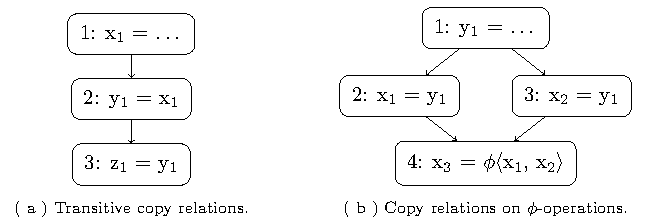
\includegraphics{copy_propagation}
    \subfloat{\label{novillo:fig:copy_propagation:a}}
    \subfloat{\label{novillo:fig:copy_propagation:b}}
  \end{center}
  \vspace{-1em}
  \caption{Analysis of copy-related variables.}
  \label{novillo:fig:copy_propagation}
\end{figure}

\begin{figure}[b!]
  \begin{center}
    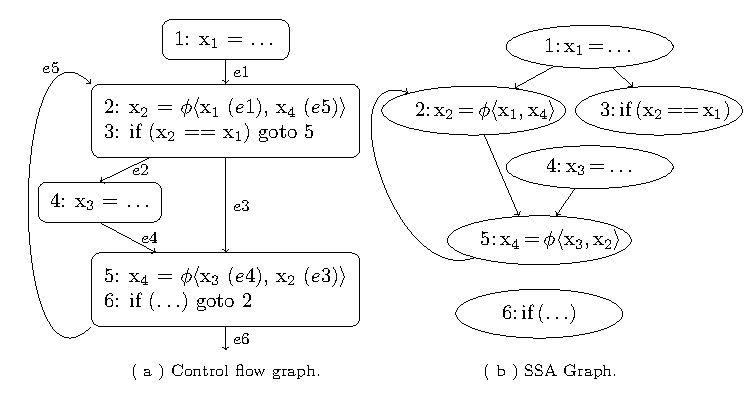
\includegraphics{copy_propagation_loop}
  \end{center}
  \vspace{-1em}
  \caption{$\phi$-operations in loops often obfuscate copy relations.}
  \label{novillo:fig:copy_propagation_loop}
\end{figure}

The analysis for copy propagation can be described as the problem of
propagating the \textit{copy-of value} of variables.  Given a sequence of
copies as shown in Figure~\ref{novillo:fig:copy_propagation:a}. We say that
y$_1$ is a \textit{copy of} x$_1$ and z$_1$ is a \textit{copy of} y$_1$.  The
problem with this representation is that there is no apparent link from z$_1$ to
x$_1$.  In order to handle transitive copy relations, all transfer functions
operate on copy-of values instead of the direct source of the copy.  If a
variable is not found to be a copy of anything else, its copy-of value is the
variable itself. For the above example, this yields that both, y$_1$ and z$_1$,
are copies of x$_1$, which in turn is a copy of itself. The lattice of this data
flow problem is thus similar to the lattice used previously for constant
propagation. The lattice elements correspond to variables of the
program instead of integer numbers. The least element of the lattice
represents the fact that a variable is a copy of itself.

Similarly, we would like to obtain the result that x$_3$ is a copy of y$_1$ for
the example of Figure~\ref{novillo:fig:copy_propagation:b}. This is
accomplished by choosing the join operator such that a copy relation is
propagated whenever the copy-of values of all the $\phi$-operation's operands
match. When visiting the $\phi$-operation for x$_3$, the analysis finds
that x$_1$ and x$_2$ are both copies of y$_1$, which allows to propagate the
result that x$_3$ is a copy of~y$_1$.

The following example shows a more complex situation where copy relations are
obfuscated by loops -- see Figure~\ref{novillo:fig:copy_propagation_loop}.  Note
that the actual visiting order depends on the shape of the CFG and immediate
uses. In other words, the ordering used here is meant for illustration only.
Processing starts
at the operation labeled $1$, with both work lists empty and the data flow
information $\top$ associated with all variables:

\begin{enumerate}
\item Assuming that the value assigned to variable x$_1$ is not a copy, the data
      flow information for this variable is lowered to $\bot$, the SSA edges
      leading to operations $2$ and $3$ are appended to the \emph{SSAWorkList},
      and the control flow graph edge $e1$ is appended to the \emph{CFGWorkList}.
\item \label{novillo:copy_prop:ex:x_2} Processing the control flow edge from the
      work list causes the edge to be marked executable and the operations
      labeled $2$ and $3$ to be visited. Since, edge $e5$ is not yet known to be
      executable the processing of the $\phi$-operation yields a copy relation
      between x$_2$ and x$_1$. This information is utilized in order to
      determine which outgoing control flow graph edges are executable for the
      conditional branch. Examining the condition shows that only edge $e3$ is
      reachable and thus needs to be added to the work list.
\item Control flow edge $e3$ is processed next and marked executable for the
      first time.
      Furthermore, the $\phi$-operation labeled $5$ is visited. Due to the fact
      that edge $e4$ is not known the be executable, this yields a
      copy relation between x$_4$ and x$_1$ (via x$_2$). The condition of the
      branch labeled $6$ cannot be analyzed and thus causes its outgoing control
      flow edges $e5$ and $e6$ to be added to the work list.
\item Now, control flow edge $e5$ is processed and marked executable. Since the
      target
      operations are already known to be executable, only the $\phi$-operation
      is revisited. However, variables x$_1$ and x$_4$ have the same copy-of
      value x$_1$, which is identical to the previous result computed in
      Step~\ref{novillo:copy_prop:ex:x_2}. Thus, neither of the two work lists
      is modified.
\item Assuming that the control flow edge $e6$ leads to the exit node of the
      control flow graph
      the algorithm stops after processing the edge without modifications to
      the data flow information computed so far.
\end{enumerate}

The straightforward implementation of copy propagation, would have needed
multiple passes to discover that x$_4$ is a copy of x$_1$.  But the iterative
nature of the propagation along with the ability to discover non-executable
code allows to handle even obfuscated copy relations. Moreover, this kind of
propagation will only reevaluate the subset of operations affected by newly
computed data flow information instead of the complete control flow graph once
the set of executable operations has been discovered.

%%%%%%%%%%%%%%%%%%%%%%%%%%%%%%%%%%%%%%%%%%%%%%%%%%%%%%%%%%%%%%%%%%%%%%%%%%%%%%%%
\section{Further Reading}
\label{novillo:sec:further_reading}

% FERNANDO: There is a lot of redundancy between this section and the
% equivalent section in Chapter \ref{chap:ssi}. I guess some refactoring can
% be used to make the final text less repetitive.

Traditional data flow analysis is well established and well described in
numerous papers. The book by Nielsen, Nielsen, and
Hankin~\cite{novillo:bib:NNH99} gives an excellent introduction to the
theoretical foundations and practical applications.
For reducible flow graphs the order in which operations are processed by the
work list algorithm can be
optimized~\cite{novillo:bib:HU73,novillo:bib:KU76,novillo:bib:NNH99}, allowing
to derive tighter complexity bounds. However, relying on reducibility is
problematic, because the flow graphs are often \emph{not} reducible even for
proper structured languages, e.g., reversed control flow graphs for backward
problems can be, and in fact almost always are, irreducible even for programs
with reducible control flow graphs. Furthermore, experiments have shown that the
tighter bounds not necessarily lead to improved compilation
times~\cite{novillo:bib:CTK06}.

Apart from computing a fixed point (MFP) solution, traditional data flow
equations can also
be solved using a more powerful approach called the \emph{meet over all paths}
(MOP) solution, which computes the \emph{in} data flow information for a basic
block by examining \emph{all} possible paths from the start node of the control
flow graph. Even though more powerful, computing the MOP solution is often
harder or even undecidable~\cite{novillo:bib:NNH99}. Consequently,
the MFP solution is preferred in practice.

The sparse propagation engine, as presented in the chapter, is based on the
underlying properties of SSA form. Other intermediate representations offer
similar properties. \emph{Static Single Information} form
(SSI)~\cite{novillo:bib:S05} allows both backward and forward problems to be
modeled by introducing $\sigma$ operations, which are placed at program points
where data flow information for backward problems needs to be
merged~\cite{novillo:bib:S04}. Bod\'{\i}k uses an extended SSA form, $e$-SSA,
to eliminate array bounds checks~\cite{novillo:bib:BGV00}.
Ruf~\cite{novillo:bib:R95} introduces the \emph{value dependence graph}, which
captures both control and data dependencies. He derives a sparse representation
of the input program, which is suited for data flow analysis, using a set of
transformations and simplifications.

The \emph{sparse evaluation graph} by Choi~et.al~\cite{novillo:bib:CCF91} is
based on the same basic idea as the approach presented in this chapter,
intermediate steps are eliminated by by-passing irrelevant CFG nodes and
merging the data flow information only when necessary. Their approach is closely
related to the placement of $\phi$-operations and similarly relies on the
dominance frontier during construction. A similar approach, presented by Johnson
and Pingali~\cite{novillo:bib:JO93}, is based on single-entry/single-exit
regions. The resulting graph is usually less sparse, but is also less complex to
compute. Ramalingam~\cite{novillo:bib:R02} further extends these ideas and
introduces the \emph{compact evaluation graph}, which is constructed from the
initial CFG using two basic transformations. The approach is superior to the
sparse representations by Choi~et.al as well as the approach presented by
Johnson and Pingali.

The previous approaches derive a sparse graph suited for data flow analysis
using graph transformations applied to the CFG.
Duesterwald~et.al~\cite{novillo:bib:DGS94} instead examine the data flow
equations, eliminate redundancies, and apply simplifications to them.

